%!TEX root=../GaugeCNNTheory.tex


\section{Rotation equivariant CNNs on punctured Euclidean spaces}
\label{sec:instantiations_euclidean_polar}

\begin{figure}
    \centering
    \begin{subfigure}[b]{0.47\textwidth}
        \centering
        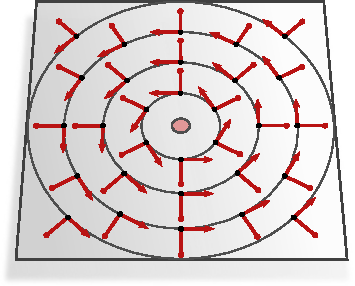
\includegraphics[width=.7\textwidth]{figures/G_structure_R2_no_origin_SO2.pdf}
        \captionsetup{format=hang, width=.82\textwidth}
        \caption{\small
            $\SO2$-invariant $\{e\}$-structure as implicitly assumed by \citet{finzi2020generalizing}.
        }
        \label{fig:G_structure_R2_no_origin_SO2}
    \end{subfigure}
    \hfill
    \begin{subfigure}[b]{0.47\textwidth}
        \centering
        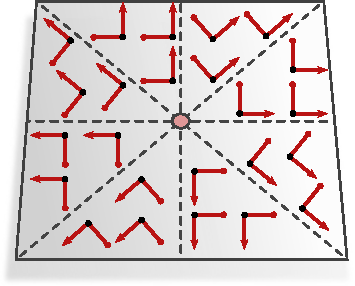
\includegraphics[width=.7\textwidth]{figures/G_structure_R2_no_origin_C8.pdf}
        \captionsetup{format=hang, width=.78\textwidth}
        \caption{\small
            $\C8$-invariant $\{e\}$-structure as implicitly assumed by \citet{chidester2019rotation}.
        }
        \label{fig:G_structure_R2_no_origin_C8}
    \end{subfigure}
    \caption{\small
        Two examples of $\{e\}$-structures on the punctured plane $\Euc_2 \backslash \{0\}$ which
        1) are invariant under rotations around the origin $\{0\}$ and
        2) consist of orthonormal frames relative to the standard Euclidean metric.
        The corresponding $\GM$-convolutions are rotation equivariant but not translation equivariant (in fact, $\Euc_2 \backslash \{0\}$ does not even admit translations).
    }
    \label{fig:G_structures_R2_no_origin}
\end{figure}


The models in rows (27-30) of Table~\ref{tab:network_instantiations}
provide an interesting alternative for rotation equivariant convolutions on punctured Euclidean spaces $\Euc_d\backslash\{0\}$.
They rely on \emph{$G$-structures that are invariant under rotations around the chosen origin $\{0\}$}, as visualized for instance in Fig.~\ref{fig:G_structures_R2_no_origin}.
By specifying a preferred origin, these models lose the property to be translation equivariant.%
\footnote{
    This issue can be resolved by combining the network with a translation invariant origin predictor network~\cite{esteves2017polar}.
    Note that the rotation equivariance of the combined model is only preserved if this origin predictor is $\SE{d}$-equivariant.
}
However, if the $G$-structure is additionally invariant under scaling, which is for instance the case when it is induced by hyperspherical coordinates with a logarithmic radial component as shown in Fig.~\ref{fig:G_structure_R2_no_origin_logpolar}, the models become equivariant w.r.t. the direct product $\SO{d} \!\times\! \Scale$ of the rotation and scaling group.
Similarly, rotation and reflection invariant $G$-structures, visualized in Fig.~\ref{fig:G_structure_R2_no_origin_O2}, imply the $\O{d}$-equivariance of the corresponding $\GM$-convolutions.


The models relate to spherical CNNs, discussed in Section~\ref{sec:instantiations_spherical} below, in two ways.
Firstly, they assume rotationally invariant $G$-structures on $\Euc_d \backslash \{0\} \,\cong\, S^{d-1} \!\times \R^+$, which can be seen as being composed of multiple rotationally invariant $G$-structures on ${(d -\! 1)}$-dimensional spherical shells $S^{d-1}$ at different radii.
The models can therefore be thought of as (hyper)spherical CNNs with an additional radial dimension~$\R^+$~\cite{ramasinghe2019representation}, which is in Fig.~\ref{fig:G_structure_R3_no_origin} visualized for the case of $d=3$ dimensions.
Secondly, the polar coordinate systems of \cite{esteves2017polar,finzi2020generalizing,chidester2019rotation} (Figs.~\ref{fig:G_structures_R2_no_origin} and~\ref{fig:G_structure_R2_no_origin_logpolar}) induce $G$-structures that exhibit the same type of singularity at their origin like those of the punctured spherical CNNs in Fig.~\ref{fig:G_structure_S2_2} at the poles.
Note that the punctured Euclidean plane $\Euc_2 \backslash \{0\}$ and the punctured sphere $S^2 \backslash \{n,s\}$ (with north and south poles $\{n,s\}$ removed) are both topologically equivalent to a cylinder $S^1 \times \R^+ \cong S^1 \times \R$ and that the cylindrical $\{e\}$-structures visualized in Figs.~\ref{fig:G_structure_R2_no_origin_SO2}, \ref{fig:G_structure_R2_no_origin_logpolar} (left) and~\ref{fig:G_structure_S2_2} are diffeomorphic.


A major difference in comparison to the $\SE{d}$-equivariant networks from the previous section is that the models of the current section are only \emph{globally} $\SO{d}$-equivariant around the origin instead of \emph{locally} $\SO{d}$-equivariant ($\SO{d}$-steerable).
While the globally equivariant models do not require $\SO{d}$-steerable kernels, they still require at least $\SO{d-1}$-steerable kernels.
This is the case since $\SO{d}$ is a $\SO{d-1}$-bundle over the spherical shells $S^{d-1} \cong \SO{d}/\SO{d-1}$ on which the $G$-structure is required to be $\SO{d}$ rotation equivariant.
For $d=2$ this allows for $\{e\}$-structures and non-steerable kernels since $\SO{d-1} = \SO{1} = \{e\}$; see Fig.~\ref{fig:G_structures_R2_no_origin} or~\ref{fig:G_structure_R2_no_origin_logpolar}.
For $d=3$ this requires at least a $\SO{d-1} = \SO{2}$-structure on the individual spherical shells, which is visualized in Fig.~\ref{fig:G_structure_S2_1}.


After these general remarks we will in the following briefly review the individual models on $\Euc_d \backslash \{0\}$ found in the literature from the viewpoint of coordinate independent CNNs.
We start with the models in row~(27) of Table~\ref{tab:network_instantiations}, which are equivariant w.r.t. $\SO2$ rotations around a chosen origin of~$\Euc_2$ and proceed with the models in row~(28), which are additionally scale equivariant.
The network listed in row~(29), which we discuss last, is globally $\O3$-equivariant around the origin of~$\Euc_3$.

